Nach dem Konzept wird nun dessen konkrete Umsetzung behandelt,
um einen tieferen Einblick in die Funktionsweise des Newsboard zu geben.

\subsection{Technische Basis}
Umgesetzt wird das Newsboard in Java, sowohl wegen persönlicher Präferenzen der Autoren,
sowie der Tatsache, dass hauptsächlich Java als Programmiersprache
an der FH Bielefeld gelehrt wird. So werden der Weiterentwicklung des Newsboards
durch weitere Studenten keine vermeidbaren Hürden in den Weg gestellt.
Darüber hinaus gibt es für Java eine große Zahl an ausgereiften
und gut dokumentierten Bibliotheken, sowie verlässliche Frameworks zum 
Build-Management. Verwendet wird das aktuelle Feature-Level von Java 8,
da es keinerlei Altlasten gibt, auf die Rücksicht genommen werden müsste.

Als Basis für das Newsboard wird das Spring-Framework im Zusammenspiel mit Maven
als Build-Management-Tool verwendet. Diese Kombination ist in der Praxis bewährt,
ist flexibel für verschiedenste Anwendungsfälle, sowie ohne große Einarbeitungszeit
gut zu benutzen. Außerdem besteht so keinerlei Bindung
an eine bestimmte Entwicklungsumgebung.

Spring bietet außerdem eine sehr ausgereifte Inversion-of-Control bzw.
Dependency Injection, wodurch eine lose Kopplung der einzelnen Komponenten
untereinander gewährt wird\cite{fowler-ioc}.
In der Umsetzung von Spring werden dabei die einzelnen Klassen nur mit
Annotationen versehen und haben ansonsten keine zwingenden Abhängigkeiten
zum Spring Framework.

Darüber hinaus können neben konkreten Klassen auch Abhängigkeiten zu Interfaces
injiziert werden, welche wiederum in ihrer Auflösung in konkrete Klassen
durch die Konfiguration von Spring beeinflusst werden können.
So kann zum Beispiel entweder eine Konfiguration für eine SQL-Datenbank,
oder einen anderen Datenspeicher angelegt werden und in Abhängigkeit
der aktivierten Konfiguration wird eine andere Implementierung für das
Interface injiziert.

\subsection{Datenmodell}
Das Datenmodell des Newsboards wird mit dem relationalen Datenbankmanagementsystem MySQL
abgebildet. Als weitverbreitetes Open-Source Produkt eignet es sich optimal, um im
Newsboard eingesetzt zu werden. Basierend auf dem vom ERD beschriebenen Modell
(Abb. \ref{fig:erd}) des Newsboards wurde ein physisches Modell für MySQL entwickelt
(Abb. \ref{fig:physical_model}).

\begin{figure}[h]
	\centering
	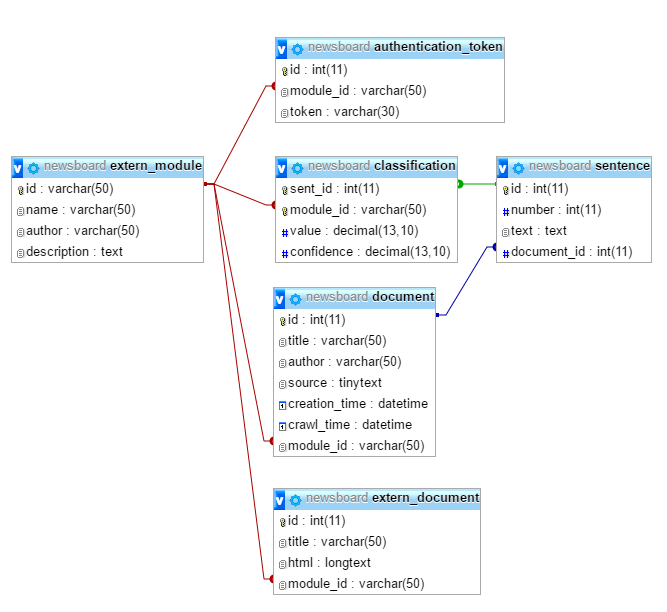
\includegraphics[scale=0.8]{content/physical-model.png}
	\label{fig:physical_model}
	\caption{Physisches Modell des Newsboards}
\end{figure}

Das Modell wird in der Schnittstelle über acht Klassen abgebildet (Abb. 
\ref{fig:uml_model}). Hier zeigen sich Abweichungen zum physischen Modell. So ist die Klasse
Document eine Containerklasse, die die Metainformationen und die Sätze des Dokuments
speichert. Um die Metainformationen eines Dokumentes zu struktieren, ist für sie eine eigene
Klasse vorhanden: DocumentMetaData. Für Sätze steht die Klasse Sentences bereit, die zudem
eine Liste mit allen Klassifikationen eines Satzes beinhaltet. Die  Klasse RawDocument dient
rein zum Einlesen von Dokumenten, welche von Crawlern bereitgestellt werden. Sie besteht aus
den Metainformationen und dem Text eines Dokumentes. Nach dem Einlesen wird ein RawDocument
in ein Document überführt.

\begin{figure}[h]
	\centering
	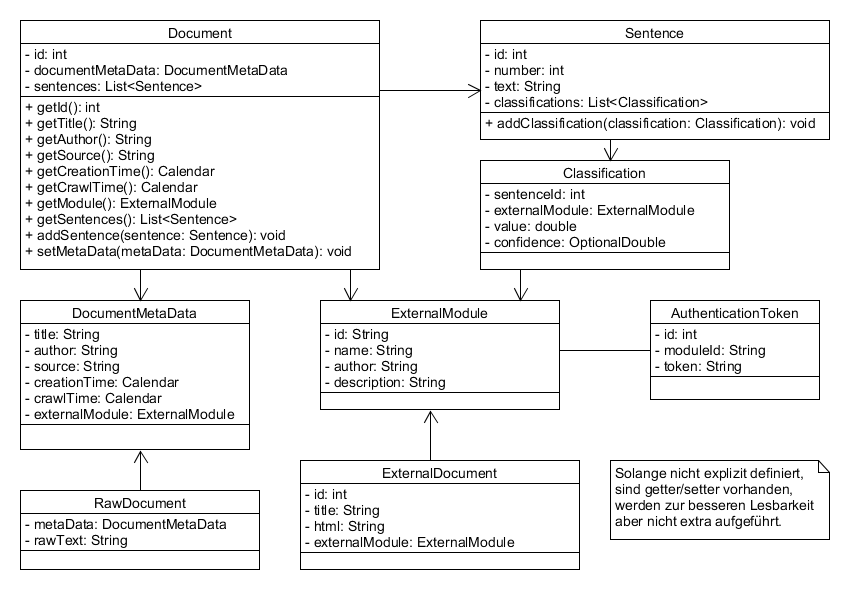
\includegraphics[scale=0.5]{content/uml-model.png}
	\label{fig:uml_model}
	\caption{Diagramm der intern verwendeten Modellklassen}
\end{figure}

Für die Kommunikation zwischen der Schnittstelle und der Datenbank wird auf das Data-
Access-Object Design Muster gesetzt, um eine hohe Modularität und Flexibilität zu
gewährleisten \cite{dao-pattern}. Beim DAO Muster werden verschiedene Interfaces
verwendet, um den Zugriff auf Datenbankoperationen zu maskieren, während die eigentliche
Übertragungslogik pro Datenquelle eigens entwickelt werden kann. Das, und die
Dependency-Injection-Funktion Springs ermöglicht es, im Falle eines Datenbankwechsels von
MySQL hin zu einem beliebigen anderem System, die Schnittstelle fast ohne Anpassungen
weiter verwenden zu können.

\subsection{Dokumentverarbeitung}
Um die RawDocuments, die die Crawler über die REST-Schnittstelle bereitstellen,
in Document-Objekte zu überführen, muss der Text in einzelne Sätze überführt werden.
Diesemn Zweck erfüllt die Klasse RawDocumentProcessor. Sie nutzt die
Apache openNLP Bibliothek, um den Plaintext von RawDocuments in Sentences zu überführen.

Apache openNLP ist eine Sammlung verschiedener Werkzeuge, um mit Java einfach diverse 
NLP-Probleme zu lösen \cite{opennlp}. Es liefert neben unterschiedlichen 
Machine-Learning-Algorithmen auch fertige Modelle zur Verwendung mit, unter anderem
zum Finden von einzelnen Sätzen. Diese Modelle sind in verschiedenen Sprachen vorhanden,
für das Newsboard wird eines zur Erkennung der deutschen Sprache genutzt.

OpenNLP stellt zur Satzerkennung das Interface SentenceDetector und die davon ableitende
Klasse SentenceDetectorME zur Verfügung. SentenceDetectorME nutzt ein Maximum-Entropy-Modell
zur Klassifizierung von Satzzeichen, die einen Satz beenden. Sie wird auch im
RawDocumentProcessor eingesetzt. Über einen einfachen Methodenaufruf kann so ein kompletter
Text verarbeitet werden. Auch die Kopplung zu openNLP bleibt sehr gering, da die
Bibliothek nur hier Verwendung findet.

\subsection{Schnittstelle}
Zur Implementierung der REST-Endpoints der Schnittstelle werden die in Spring enthaltenen
Controller-Features genutzt. Um damit einen Endpoint zu bedienen, reicht es aus,
eine Methode innerhalb einer Controller-Klasse mit \texttt{RequestMapping} zu annotieren.
Listing \ref{lst:restExample} zeigt Beispielhaft, wie ein solcher Endpoint unter Angabe der
Annotations-Parameter implementiert werden kann.

Der Rückgabewert der Methode wird so direkt als Antwort an den Client zurückgeliefert.
Darüber hinaus können mit Hilfe der Dependency-Injection von Spring weitere Parameter
definiert werden, die z.B. die HTTP-Anfrage, oder die Antwort wie im Beispiel.
\vspace{1em}

\begin{java}{Implementierung eines REST-Endpoints mit Spring}{lst:restExample}
@RestController
public class RestApiController {
	[...]
	@RequestMapping(path = "/document", method = RequestMethod.GET, produces = MediaType.APPLICATION_XML_VALUE)
	public String listDocuments(HttpServletResponse response) {
		[...]
		return documents;
	}
	[...]
}
\end{java}

Auf diese Weise werden jeweils die im Konzept aufgezählten Aktionen implementiert.
Es ergeben sich zur wesentlichen Vereinfachung der Benutzung der Schnittstelle,
sowie um möglichst effektiv arbeiten zu können, mehrere Endpoints zum Lesen
der Dokumente. Insgesamt ergibt sich somit die folgende Liste an vorhandenen
Kombinationen von Aktionen und Ressourcen:

\begin{itemize}
	\item \textbf{GET /document}
	Lesen einer Liste der Metadaten aller Dokumente
	\item \textbf{GET /document/\{id\}}
	Lesen eines vollständigen, spezifizierten Dokuments inklusive
	einzelnen Sätzen und Klassifikationen
	\item \textbf{PUT /document}
	Einfügen eines neuen Dokuments durch einen Crawler
	\item \textbf{GET /unclassified}
	Lesen aller Dokumente, die vom aktuell authentifizierten Classifier
	noch nicht bewertet wurden
	\item \textbf{PUT /classify}
	Einfügen neuer Klassifizierungen durch einen Classifier
\end{itemize}

Um die Ressourcen der REST-Schnittstelle klar von der Web-Oberfläche zu trennen,
sind die angegebenen Pfade relativ zum Verzeichnis \texttt{/rest}.

Da nicht jeder beliebige Nutzer neue Dokumente oder Klassifizierungen einfügen
können soll, muss eine Art von Authentifizierung vorhanden sein.
Es bietet sich an, auch der Lesen von unklassifizierten Dokumenten nur authentifizierten
Nutzern zugänglich zu machen, da dies immer spezifisch
für einen bestimmten Classifier ist.
Umgesetzt wird dies mit einer HTTP-Basic Authentifizierung, die sehr einfach umzusetzen
ist, aber für die vorgesehenen Einsatzzwecke ausreicht.
Als Benutzername dient immer die ID des Crawlers oder Classifiers, die in der Datenbank hinterlegt ist. Als Passwort dient ein in der Datenbank hinterlegtes AuthenticationToken.

\subsection{XML-Format}
Über die REST-Endpoints hinaus ist bei der Schnittstelle noch die Verarbeitung
der XML-Daten, sowie das Schema zur Validierung interessant.
Da die zu erwartenden Datenmengen im Vorhinein nicht abschätzbar sind,
sollte das Lesen und vor allem das Schreiben der XML-Daten möglichst wenig Speicher
verbrauchen, um eventuelle Engpässe zu vermeiden. Beim Lesen ist eine Validierung
gegen das Schema unbedingt notwendig, da nicht davon ausgegangen werden kann,
dass die ankommenden Daten in jedem Fall valide sind.

Aufgrund der Speicheranforderungen ist ein herkömmlicher DOM-Parser in diesem Projekt
nicht geeignet. Gelesen werden die XML-Daten stattdessen mit einem SAX-Parser\cite{insel-xml}. Dieser ist weniger Speicher belastend als ein DOM-Parser
und kann, anders als ein StAX-Parser eine Validierung des Dokuments während
des Einlesens durchführen. Verwendet wird die Standard Implementierung
des JDK: \texttt{javax.xml.parsers.SAXParser}.

Da SAX-Parser üblicherweise nur lesen, aber nicht schreiben können, kommt dazu ein
anderer Parser zum Einsatz. In diesem Fall ein StAX-Parser,
da Validierung nicht zwingend zur Laufzeit erfolgen muss, sondern im Vorhinein
im Zuge automatisierter Tests durchgeführt werden kann.
Verwendet wird hier ebenfalls eine Implementierung, die Bestandteil des JDK ist:
\texttt{javax.xml.stream.XMLStreamWriter}.
Um die genauere Arbeitsweise beim Verarbeiten der XML-Daten zu beschreiben,
wird an dieser Stelle das erstellte Schema beschrieben.

Das im Schema spezifizierte XML-Format erlaubt Dokumente verschiedenster Ausprägung.
Das ist notwendig, damit einerseits nicht mehrere Schemata angelegt und gepflegt
werden zu müssen, und andererseits die Anforderungen der verschiedenen
REST-Endpoints erfüllt werden.

Das Schema ist so spezifiziert, dass jedes XML-Dokument eine Liste von Dokumenten
im Sinne des Datenmodells enthalten kann.
Dabei kann jedes Dokument Metadaten enthalten (z.B. Autor, Quelle), die beim Einlesen
neuer Dokumente und beim Ausgeben vorhandener Dokumente vorhanden sein müssen.
Dazu kommt entweder ein Element mit Rohtext beim Einfügen der Dokumente,
oder eine Liste von Sätzen und Klassifikationen.

Die Sätze sind nur beim Ausgeben von Dokumenten wichtig, beim Einlesen
neuer Klassifikationen sind sie, wie die Metadaten auch,
optional und werden nicht beachtet.
Wenn eine Liste von Sätzen vorhanden ist, muss sie mindestens einen Satz enthalten.
Die Liste von Klassifikationen ist beim Ausgeben spezifizierter
und unklassifizierter Dokumente von Belang, sowie natürlich
beim Einlesen neuer Klassifikationen. Da z.B. bei frisch eingelesenen Dokumenten noch keine Klassifizierungen vorliegen können, darf die Liste auch leer sein.

Um das Arbeiten mit diesen Dokumenten deutlich zu vereinfachen, können XML-Dokumente
weder in beliebiger Ausprägung geschrieben noch gelesen werden. Stattdessen können
nur XML-Daten eingelesen werden, wie sie zum Einfügen neuer Dokumente
oder Klassifizierungen benötigt werden.
Geschrieben werden können nur Dokumentenausschnitte (intern Stub genannt),
die nur Metadaten beinhalten, und vollständige Dokument-Strukturen ausgegeben werden.

\subsection{Web-Oberfläche}
Um das Newsboard über die REST-Schnittstelle hinaus auch für Benutzer verfügbar zu machen,
beinhaltet es eine einfache Web-Oberfläche.
Diese ist im jetzigen Zustand nur im Stande, eine Liste von klassifizierten Dokumenten,
oder eine Detailseite zu einem einzelnen Dokument anzuzeigen.

Auf der Übersichtsseite werden nur Titel, Inhalt und ein berechneter Durchschnittswert
aller Klassifikationen zu einem Dokument angezeigt. Auf der Detailseite werden
darüber hinaus noch weitere Metadaten, wie Quelle, Crawler, Einzesezeitpunkt
und wenn verfügbar auch Autor und Veröffentlichungsdatum angezeigt.

Die Durchschnittsberechnung ergibt sich, indem zu jedem Satz einzeln ein Durchschnitt berechnet wird und anschließend das arithmetische Mittel Aller Satzbewertungen
gebildet wird. Die Satzbewertungen werden berechnet, indem ebenfalls das arithmetische Mittel aller vorliegenden Bewertungen gebildet wird. Falls vorhanden wird dabei allerdings
auch der confidence-Wert mit einbezogen, indem er mit dem jeweiligen Klassifikationswert
multipliziert wird.

Bei der Oberfläche handelt es sich um eine klassische, serverseitig Generierte.
Dabei wird die Thymeleaf-Templage-Engine verwendet, für die es eine einfach Integration in
Spring gibt. Sie verfolgt den sogenannten "`Natural Templating"'-Ansatz,
bei dem die HTML-Templates auch in ihrer Rohfassung korrekt von einem Browser
dargestellt werden können. Dadurch ist allerdings das Ausgabeformat
auf HTML-Dialekte beschränkt.

Um die Oberfläche mit geringem zusätzlichen Aufwand optisch ansprechend zu gestalten,
kommt das Bootstrap-Framework zum Einsatz. Es wird von Twitter entwickelt und
beinhaltet viele Möglichkeiten, Layout zu gestalten und einfache Inhalte
ansehnlich darzustellen\cite{bootstrap}.

\subsection{Testing}
Um eine korrekte Funktion des Newsboard zu gewährleisten und möglichst früh
Fehler zu erkennen, wurde zu großen Teilen testgetrieben entwickelt.
Als Testing-Framework kam Spock zum Einsatz. Es bietet gegenüber JUnit einige Vorteile,
wie das Strukturieren von Testfällen in given/when/then-Blöcke,
oder das, durch die Programmierung in Groovy ermöglichte, Testen privater Methoden
außerhalb der entsprechenden Klassen.

Zusätzlich kam das Jacoco-Maven-Plugin zum Einsatz, um die Testabdeckung des Newsboards
zu messen. In der finalen Fassung liegt die Zeilenabdeckung bei 92\%
und die Entscheidungsabdeckung bei 76\% für das gesamte Projekt.
Für die Model-Klassen besteht darüber hinaus vollständige Zeilenabdeckung,
sowie 89\% Entscheidungsabdeckung. Dabei ist zu beachten, dass JaCoCo einige Pfade
mit einberechnet, die sich gegenseitig ausschließen, und entsprechend
nicht abgedeckt werden können. Ein Beispiel dafür ist die oder-verknüpfte Abfrage
auf Null und eine Klassenzugehörigkeit, die mehrfach in \texttt{equals}-Methoden vorkommt.
